\documentclass{ou-report}
\citestyle{agu}

% Dit template is gemaakt door P.J. Molijn in het kader van zijn afstuderen aan de OU in 2014.
% Waarvoor hartelijk dank.
% Minieme maar belangrijke wijzigingen zijn aangebracht door E.M. van Doorn
% Het template is versimpeld door Sylvia Stuurman, 2019.


%\hypersetup{
%pdfsubject={Master Thesis <Titel>, <author>},
%pdfkeywords={keyword1, keyword2}
%}

\begin{document}
\pagestyle{plain}
\title{Dit is de titel van mijn}
\author{Tjibbe van der Ede}
%Title of the thesis
%\title[Subtitle]{Title}
%\author{author}
%\affiliation{
%\begin{tabular}{ll}
%Student: & studentnumber \\
%Date:    & DD/MM/YYY \\
%\end{tabular}
%}
%
%%\coverimage{cover/cover.jpg}
%%            ===============
%\makecover[frontboxwidth=4.6in]
\begin{titlepage}

    \begin{center}

        %% Insert the OU logo at the bottom of the page.
        \begin{tikzpicture}[remember picture,overlay]
            \node at (current page.south)[anchor=south,inner sep=0pt]{
                
\includegraphics[scale=0.7]{cover/logo}
            };
        \end{tikzpicture}

        %% Extra whitespace at the top.
        \vspace*{2\bigskipamount}

        %% Print the title in specific color.
        {\makeatletter
            %\titlestyle\color{ou-cyan}\Huge\@title
            \titlestyle\color{red}\Huge\@title
            \makeatother}

        %% Print the optional subtitle in black.
        {\makeatletter
            \ifx\@subtitle\undefined\else
                \bigskip
                \titlefont\titleshape\LARGE\@subtitle
            \fi
            \makeatother}

        \bigskip
        \bigskip

        by
        %door

        \bigskip
        \bigskip

        %% Print the name of the author.
        {\makeatletter
            \titlefont\Large\bfseries\@author
            \makeatother}

        \vfill

        in partial fulfillment of the requirements for the degree of
        %in overeenstemming met de vereisten voor het verkrijgen van de graad van

        \bigskip
        \bigskip

        {\bfseries Master of Science}

        in Software Engineering

        \bigskip
        \bigskip

        at the Open University, faculty of Management, Science and Technology \\
        Master Software Engineering
        %aan de Open Universiteit Nederland,

        to be defended publicly on 12 October, 2023 at 9:30 AM.
        %in het openbaar te verdedigen op dinsdag 9 september om 15:00 uur.

        \vfill

        \begin{tabular}{lll}
            %% Add additional information here, per faculty requirements, e.g
            Student number: & 852372917                                                 \\
            Course code:    & IMA0002                                                   \\
            Thesis committee:
                            & Dr. Ir. Mina Sheikhalishahi (chairman), & Open University \\
                            & Dr. Ir. Clara Maathuis (supervisor),    & Open University
        \end{tabular}

        %% Only include the following lines if confidentiality is applicable.
        \bigskip


        \bigskip

    \end{center}

\end{titlepage}


%% Use Roman numerals for the page numbers of the title pages and table of
%% contents.
\pagenumbering{roman}
%% Include an optional title page.

\frontmatter


\let\cleardoublepage\clearpage

% Optional Dedication, Acknowledgement
%\input{dedication}

%\input{acknowledgement}
\tableofcontents

%Optional: list of figures, list of tables
%\listoffigures

%\listoftables

%% Include an optional summary page.
%\chapter{Summary}

%\input{Summary/samenvatting}

\mainmatter
\pagenumbering{arabic}

\chapter{Title of the chapter}
This is just to show how to include a test file for a chapter, a reference \cite{ledesma_scree_2015}

\chapter{Related work}
\subsection*{Distributed clustering}
Recent work for clustering is authored by Xia et al. \cite{xia_distributed_2020}.
Their work focuses specifically on a distributed variant of the K-means cluster algorithm.
They propose a method for applying LDP for distributed K-means. For this purpose, a modified LDP algorithm is proposed.
To fit K-means clustering, the features are converted to binary strings rather than boolean values. RR is then used to perturb each feature and is combined into a feature vector.
The privacy cost is dependent on the length of bits of each feature transformation. This means a longer length yields more information, at the cost of the privacy budget.
In every iteration, the data is aggregated (server-side) and the K-means algorithm calculates and sends centroids to each user.
In response, the user (client-side) re-calculates the distances until the centroid becomes stable.
The disadvantage of the approach is the high correlation between user data ($V = {v^0, v^1...v^n}$) and the clusters ($U = {u^0, u^1...u^n}$).
To solve this an enhancement to the algorithm is proposed. The client-side still sends $v^i$, but now also includes a random zero string set of $S = {z,...v^i...x}$.
The perturbed version $S'$ is sent to the server-side along with $v^i$. Now, the server-side conducts similar calculations to receive the real cluster.
\textit{research why this is not a suitable solution}. \newline
A paper written by Huang et al. \cite{9679364} extends Xia et al.'s work.
Like the previous paper, the algorithm is used for 2-dimensional distributed clustering.
The authors aim at fixing a shortcoming of the solution provided by Xia et al.
Namely, a too big difference between actual and perturbed values.
Their solution is to use Condensed Local Differential Privacy (CLDP) for small-scale values and LDP for large-scale values.
To reach CLDP a distance-aware LDP is used.
The method for the client side to calculate the distance between two values is Square Wave (SW) mechanism, which is also used for large-scale data.
Another method that also satisfies $\alpha-CLDP$ is using the Manhattan distance.
Finally, the perturbed data is used with a classical K-Means algorithm on the server-side.


\subsection*{k-anonimity}
TODO
\subsection*{Location based clustering}
The next two papers apply LDP as well, but it is more related to location mapping. However, the way they take care of the problem corresponds to clustering.
The paper written by Andrés et al. focuses on clustering for 2-dimensional data \cite{DBLP:journals/corr/abs-1212-1984}.
Especially meant for location-based systems (LBS). This location data has a big impact on privacy for individuals, which is why this paper focuses on integrating LDP with 2-d clustering. \newline
They provide a solution by perturbing real-time location data by sending a random location in the same radius $r$.
The level of privacy $l$ is dependent on the size of $r$ and $\epsilon$-geo-indistinguishability is then defined as $\epsilon=l/r$. \newline
LDP is used by randomly selecting a location on the device of a user. A set of interesting locations $X$ based on the original $x \in X$ is extracted from a GPS service.
These values are calculated based on the Euclidian distance $d(x, x')$ for which everything should be within a radius $r$.
Finally, the noise is added based on a probabilistic method $K$, which is similar to that of the Laplace distribution.
To support higher dimensions, they used the polar Laplace by using the distance. This mechanism was then further improved and named “Planar Laplace mechanism” \cite{DBLP:journals/corr/abs-1212-1984} \newline
The same mechanism could be applied to a tuple of points, by applying the distance between tuples of points.
Method $K$ can be individually applied to each point to achieve $\epsilon$-geo-indistinguishability.
The calculation of multiple locations is computationally heavy. Their current solution is to apply the technique for single locations for each location independently, but suffers from performance issues.
Therefore, future studies should research the appliance of existing methods to solve this issue. \newline \newline
Research conducted by Min et al. \cite{9646489} extends geo-indistinguishability for 3-dimensional data.
Instead of using a plane for cartesian coordinates, they use a sphere for projecting 3D coordinates (X, Y, Z).
Similar to the 2D-variant the La place algorithm was used. Therefore, in extension to $d(x, x')$ they define $d^3(x, x')$.



\subsection*{Summary}
A few papers researched privacy-oriented distributed K-means.
Their solutions yielded promising results but still needed a server in between.
Although the results were perturbed, there was still information leaked regarding cluster information.
Because K-means is a distance-based algorithm the geo-indistinguishability has shown promising results.
Notably, the paper that is written by Min et al. \cite{9646489} is very promising for K-means clustering.
This paper is recent and there is currently no research conducted for applying LDP on n-dimensional data with K-means clustering.
Therefore, this thesis will research the possibility of extending the 3-dimensional LDP to use for n-dimensional data.
And the effectiveness of this data for usage with K-means clustering.
%% based on centroids, so centroid is x1 and x0 / x2 / x3 are perturbed locations within radius R.
%% So distributed K-means. Every round new centroids are created based on this information.

\subsubsection*{Validation}
A common way of calculating the performance of LDP with K-means is calculating the error-rate against an original K-means algorithm.
One way is to calculate the Relative Error (RE) \cite{xia_distributed_2020},  \cite{9679364}.
This is calculated to measure the deviation of centroids to the actual centroids (centroids produced by non LDP K-means).
Another metric is named the adjusted mutual information (AMI) score. This score is used to quantify similarities between the original and perturbed cluster results \cite{9679364}.


%\input{Chapter2/chapter-2}

%\input{Chapter3/chapter-3}

%\input{Chapter4/chapter-4}

%\input{Chapter5/chapter-5}

%\input{Chapter6/chapter-6}



\backmatter
\pagenumbering{roman}

\bibliographystyle{plainnat}
\bibliography{report}

%% Use letters for the chapter numbers of the appendices.
%\appendix
\appendix
%  \chapter{Hyperparameters}
\section{K-Means}
For selecting the appropriate amount of clusters, we used the silhouette method. 
Using this method, we ran the K-Means method multiple times for different $k$ values.
The results are plotted using a line-plot, and we select the highest silhouette score from this plot. 
\begin{enumerate}
  \item Seeds dataset (All dimensions): k-clusters.
  \begin{enumerate}
      \item 2-dimensions k-value: 2
      \item 3-dimensions k-value: 5
      \item 7-dimensions k-value: 2
  \end{enumerate}
      \item Heart dataset:
      \begin{enumerate}
          \item 2-dimensions k-value: 2
          \item 3-dimensions k-value: 4
          \item 9-dimensions k-value: 2
      \end{enumerate}
      \item Circle dataset:
      \begin{enumerate}
          \item 2-dimensions k-value: 7
          \item 3-dimensions k-value: 9
      \end{enumerate}
      \item Line dataset:
      \begin{enumerate}
          \item 2-dimensions k-value: 2
          \item 3-dimensions k-value: 2
      \end{enumerate}
      \item Skewed dataset:
      \begin{enumerate}
          \item 2-dimensions k-value: 5
          \item 3-dimensions k-value: 4
      \end{enumerate}
  \end{enumerate}

\newpage
\subsection{Seeds dataset}
\begin{figure}[H]
  \includegraphics[width=0.75\textwidth]{Method/images//k-values/seeds-dataset-2-kmeans.png}
  \caption{Selecting the $k$ for K-Means clustering for seeds dataset (2 dimensions) using the "silhouette method"}
  \label{hyperparameters:agglomerative-seeds-dataset-2d}
\end{figure}
\begin{figure}[H]
  \includegraphics[width=0.75\textwidth]{Method/images/k-values/seeds-dataset-2-kmeans.png}
  \caption{Selecting the $k$ for K-Means clustering for seeds dataset (3 dimensions) using the "silhouette method"}
  \label{hyperparameters:agglomerative-seeds-dataset-3d}
\end{figure}
\begin{figure}[H]
  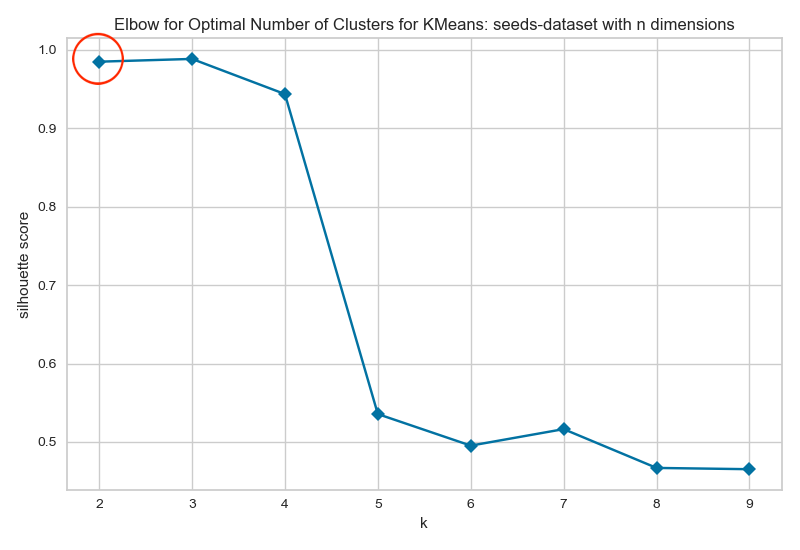
\includegraphics[width=0.75\textwidth]{Method/images/k-values/seeds-dataset-n-kmeans.png}
  \caption{Selecting the $k$ for K-Means clustering for seeds dataset (7 dimensions) using the "silhouette method"}
  \label{hyperparameters:agglomerative-seeds-dataset-7d}
\end{figure}
\newpage

\subsection{Heart dataset}
\begin{figure}[H]
  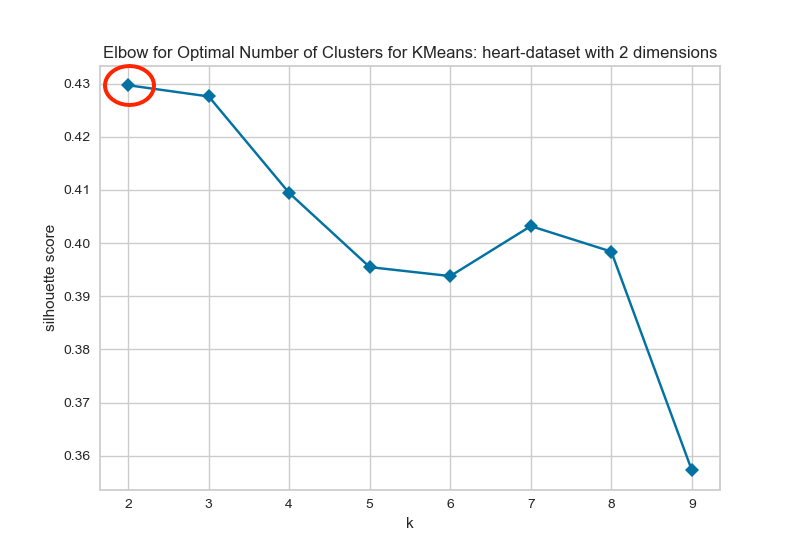
\includegraphics[width=0.75\textwidth]{Method/images/k-values/heart-dataset-2-kmeans.png}
  \caption{Selecting the $k$ for K-Means clustering for Heart dataset (2 dimensions) using the "silhouette method"}
  \label{hyperparameters:agglomerative-heart-dataset-2d}
\end{figure}
\begin{figure}[H]
  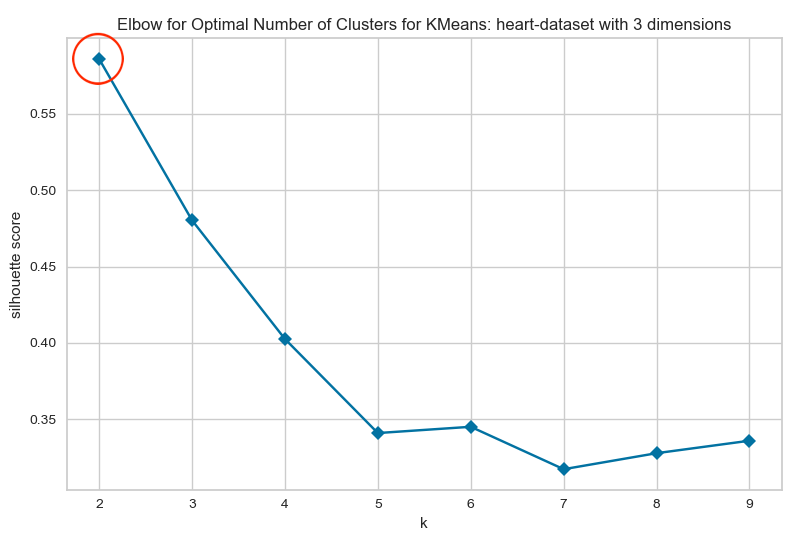
\includegraphics[width=0.75\textwidth]{Method/images/k-values/heart-dataset-3-kmeans.png}
  \caption{Selecting the $k$ for K-Means clustering for Heart dataset (3 dimensions) using the "silhouette method"}
  \label{hyperparameters:agglomerative-heart-dataset-3d}
\end{figure}
\begin{figure}[H]
  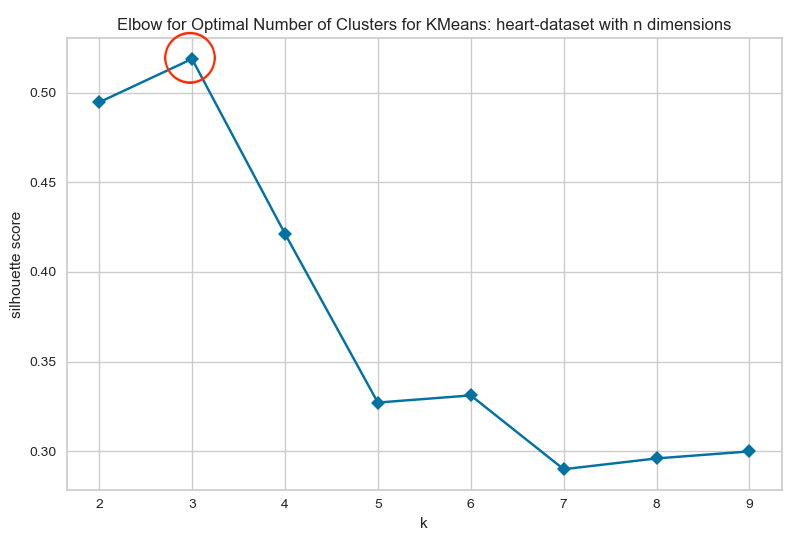
\includegraphics[width=0.75\textwidth]{Method/images/k-values/heart-dataset-n-kmeans.png}
  \caption{Selecting the $k$ for K-Means clustering for Heart dataset (9 dimensions) using the "silhouette method"}
  \label{hyperparameters:agglomerative-heart-dataset-9d}
\end{figure}
\newpage

\subsection{Circle dataset}

\begin{figure}[H]
  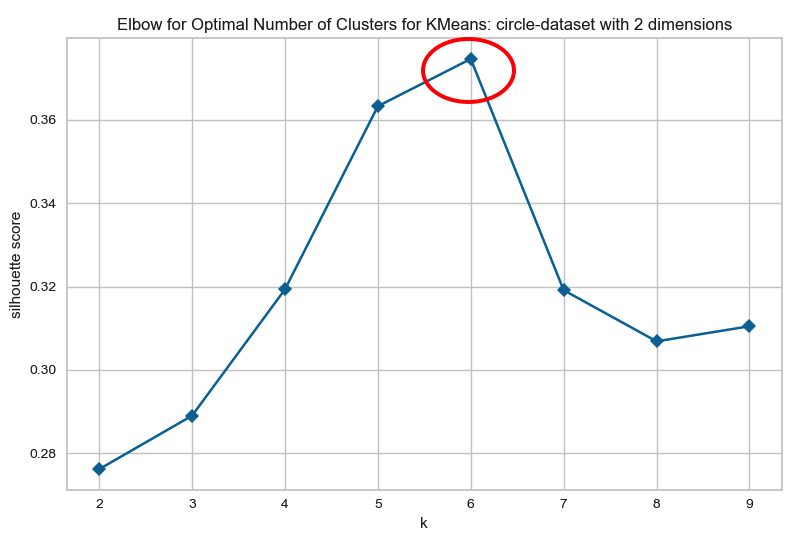
\includegraphics[width=0.75\textwidth]{Method/images/k-values/circle-dataset-2-kmeans.png}
  \caption{Selecting the $k$ for K-Means clustering for circle dataset (2-dimensions) using the "silhouette method"}
  \label{hyperparameters:agglomerative-circle-dataset-2d}
\end{figure}
\begin{figure}[H]
  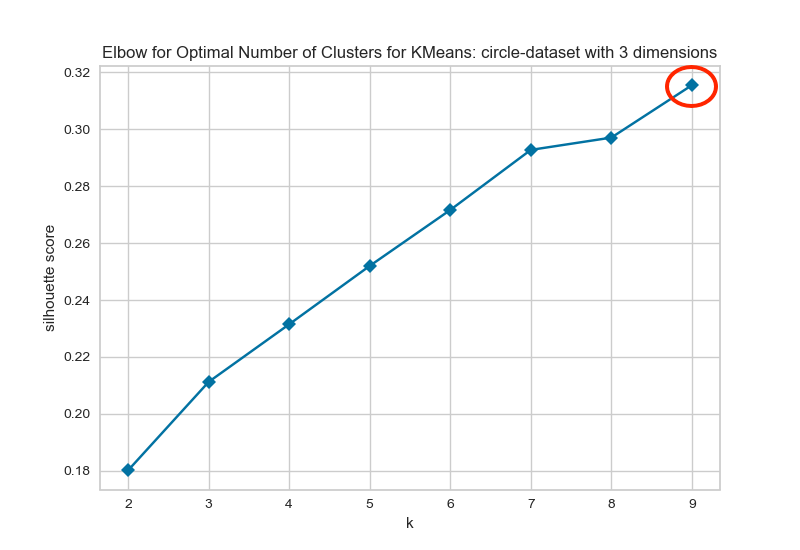
\includegraphics[width=0.75\textwidth]{Method/images/k-values/circle-dataset-3-kmeans.png}
  \caption{Selecting the $k$ for K-Means clustering for circle dataset (3-dimensions) using the "silhouette method"}
  \label{hyperparameters:agglomerative-circle-dataset-3d}
\end{figure}
\newpage

\subsection{Line dataset}
\begin{figure}[H]
  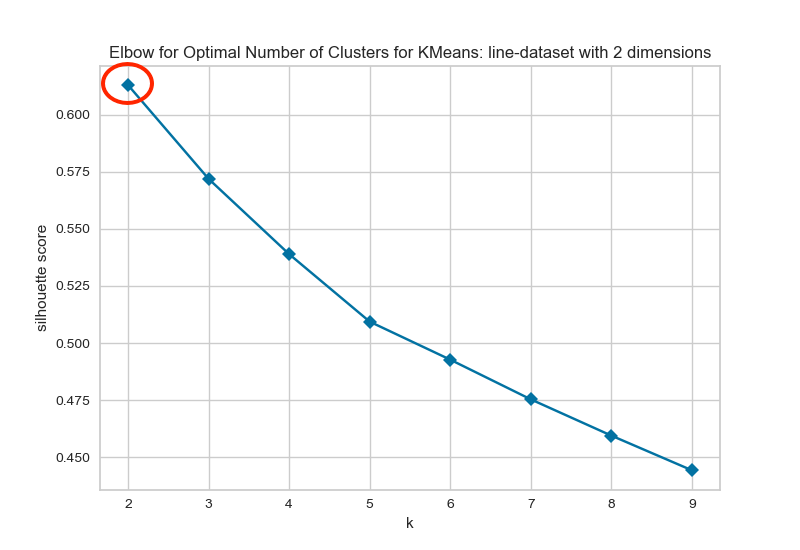
\includegraphics[width=0.75\textwidth]{Method/images/k-values/line-dataset-2-kmeans.png}
  \caption{Selecting the $k$ for K-Means clustering for line dataset (2-dimensions) using the "silhouette method"}
  \label{hyperparameters:agglomerative-line-dataset-2d}
\end{figure}
\begin{figure}[H]
  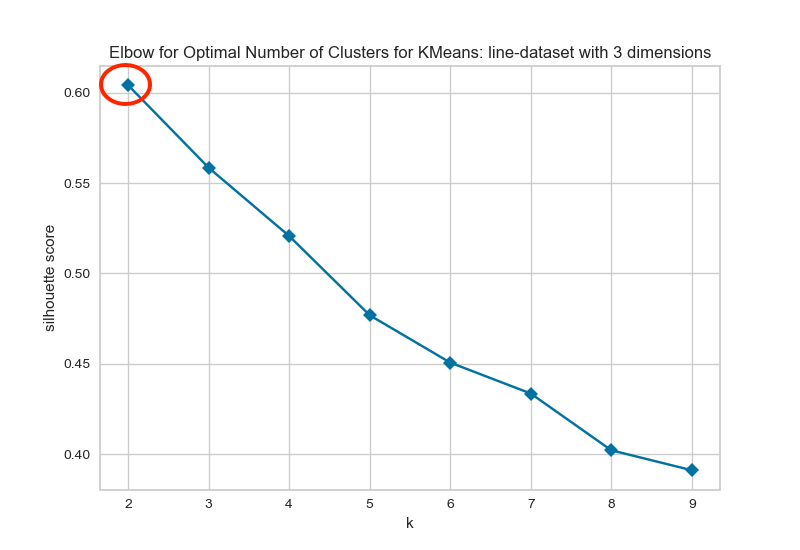
\includegraphics[width=0.75\textwidth]{Method/images/k-values/line-dataset-3-kmeans.png}
  \caption{Selecting the $k$ for K-Means clustering for line dataset (3-dimensions) using the "silhouette method"}
  \label{hyperparameters:agglomerative-line-dataset-3d}
\end{figure}
\newpage
\subsection{Skewed dataset}
\begin{figure}[H]
  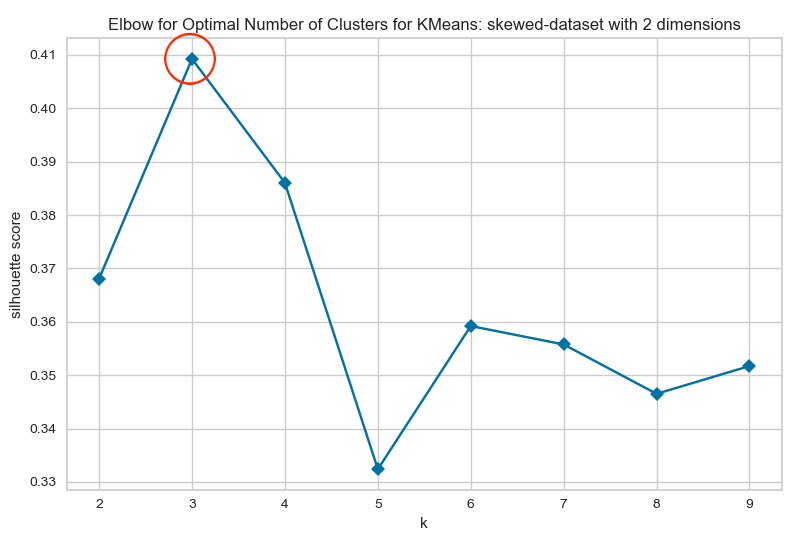
\includegraphics[width=0.75\textwidth]{Method/images/k-values/skewed-dataset-2-kmeans.png}
  \caption{Selecting the $k$ for K-Means clustering for skewed dataset (2-dimensions) using the "silhouette method"}
  \label{hyperparameters:agglomerative-skewed-dataset-2d}
\end{figure}
\begin{figure}[H]
  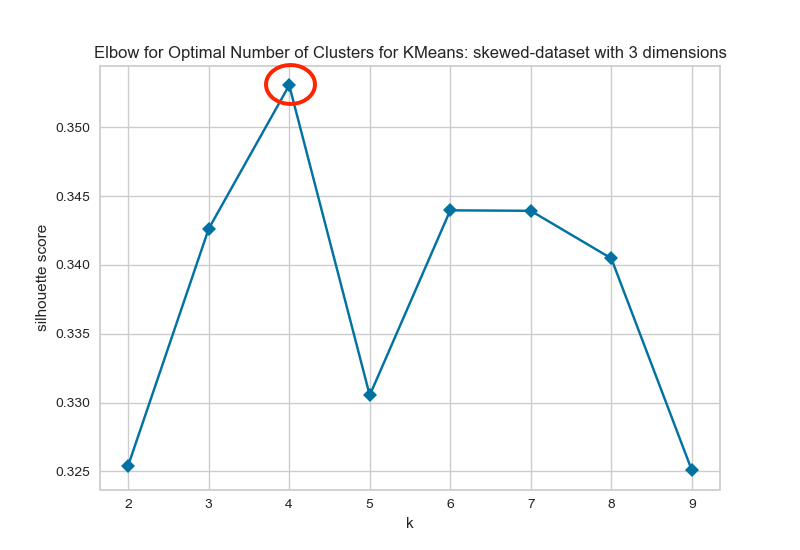
\includegraphics[width=0.75\textwidth]{Method/images/k-values/skewed-dataset-3-kmeans.png}
  \caption{Selecting the $k$ for K-Means clustering for skewed dataset (3-dimensions) using the "silhouette method"}
  \label{hyperparameters:agglomerative-skewed-dataset-3d}
\end{figure}
\newpage
\section{Agglomerative clustering} \label{appendix:agglomerative-hyperparameters}
The same as with K-Means applies to \gls{ag}.
\begin{enumerate}
    \item Seeds dataset:
    \begin{enumerate}
        \item 2-dimensions k-value: 2
        \item 3-dimensions k-value: 2
        \item 7-dimensions k-value 4
    \end{enumerate}
    \item     Heart dataset:
    \begin{enumerate}
        \item 2-dimensions k-value: 2
        \item 3-dimensions k-value: 4
        \item 9-dimensions k-value 3
    \end{enumerate}
    \item Circle dataset:
    \begin{enumerate}
        \item 2-dimensions k-value: 7
        \item 3-dimensions k-value: 9
    \end{enumerate}
    \item Line dataset (all dimensions) k-value: 
    \begin{enumerate}
        \item 2-dimensions k-value: 2
        \item 3-dimensions k-value: 3
    \end{enumerate}
    \item Skewed dataset:
    \begin{enumerate}
        \item 2-dimensions k-value: 6
        \item 3-dimensions k-value: 9
    \end{enumerate}
\end{enumerate}
\newpage
\subsection{Seeds dataset}
\begin{figure}[H]
  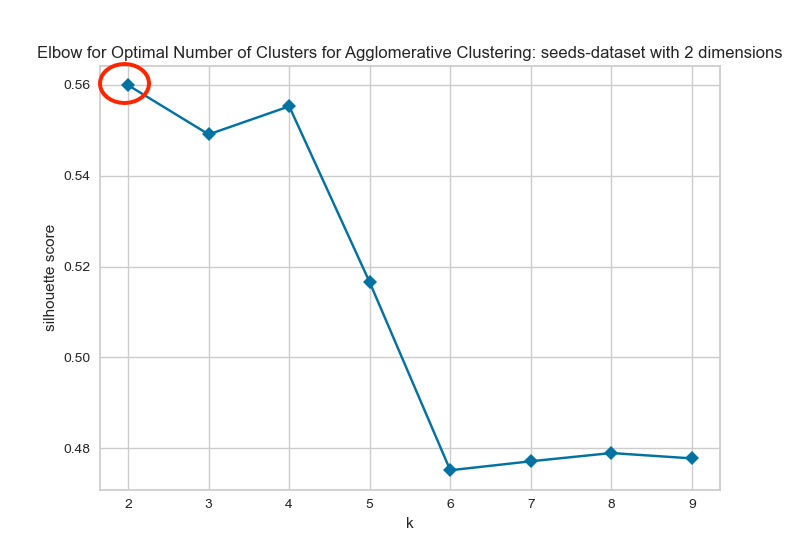
\includegraphics[width=0.75\textwidth]{Method/images/k-values/seeds-dataset-2-agglomerative.png}
  \caption{Selecting the $k$ for Agglomerative clustering for seeds dataset (2 dimensions) using the"silhouette method"}
  \label{hyperparameters:agglomerative-seeds-dataset-2d}
\end{figure}
\begin{figure}[H]
  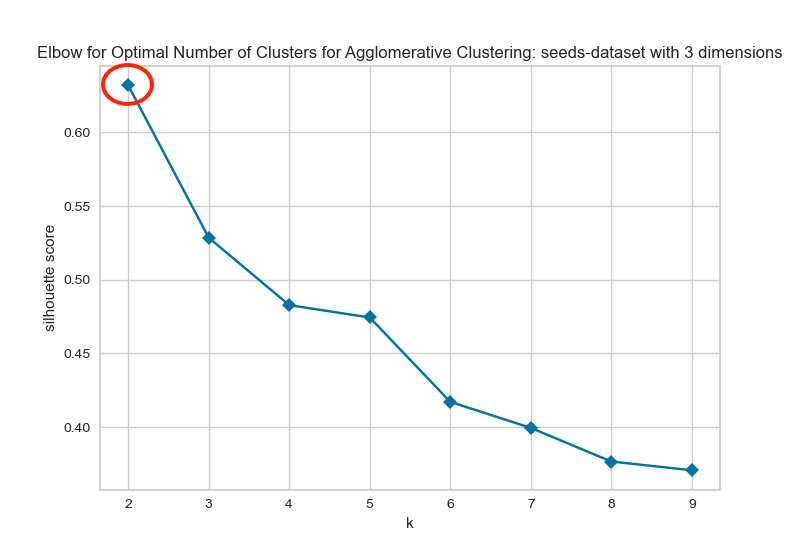
\includegraphics[width=0.75\textwidth]{Method/images/k-values/seeds-dataset-3-agglomerative.png}
  \caption{Selecting the $k$ for Agglomerative clustering for seeds dataset (3 dimensions) using the "silhouette method"}
  \label{hyperparameters:agglomerative-seeds-dataset-3d}
\end{figure}
\begin{figure}[H]
  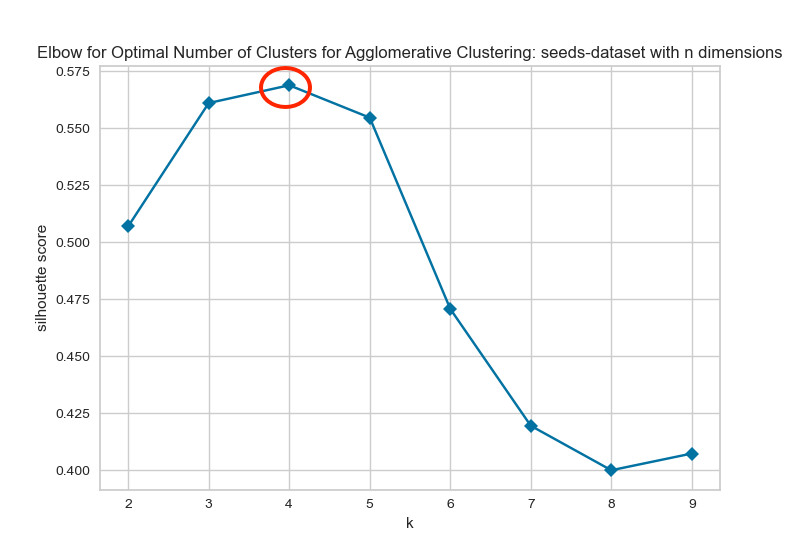
\includegraphics[width=0.75\textwidth]{Method/images/k-values/seeds-dataset-n-agglomerative.png}
  \caption{Selecting the $k$ for Agglomerative clustering for seeds dataset (7 dimensions) using the "silhouette method"}
  \label{hyperparameters:agglomerative-seeds-dataset-7d}
\end{figure}
\newpage

\subsection{Heart dataset}
\begin{figure}[H]
  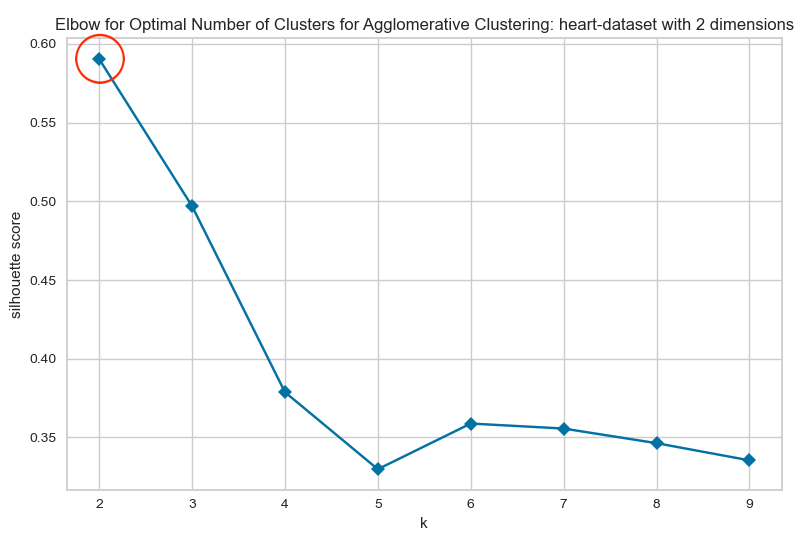
\includegraphics[width=0.75\textwidth]{Method/images/k-values/heart-dataset-2-agglomerative.png}
  \caption{Selecting the $k$ for Agglomerative clustering for Heart dataset (2 dimensions) using the "silhouette method"}
  \label{hyperparameters:agglomerative-heart-dataset-2d}
\end{figure}
\begin{figure}[H]
  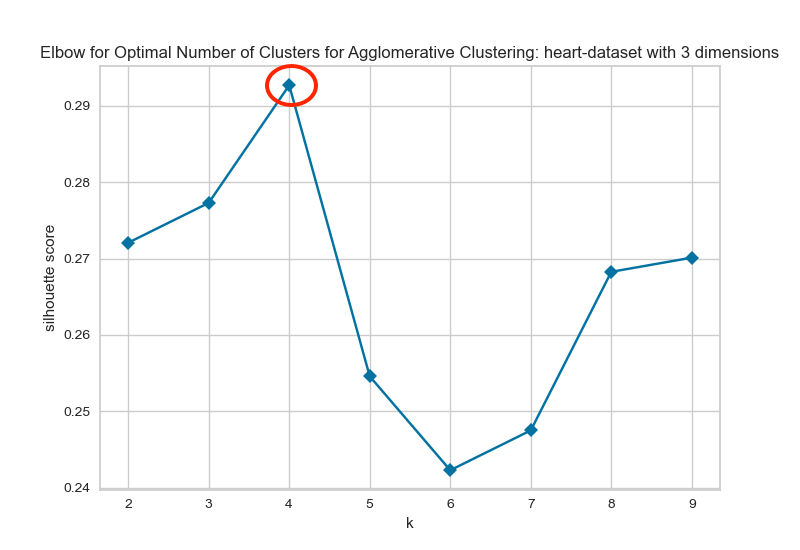
\includegraphics[width=0.75\textwidth]{Method/images/k-values/heart-dataset-3-agglomerative.png}
  \caption{Selecting the $k$ for Agglomerative clustering for Heart dataset (3 dimensions) using the "silhouette method"}
  \label{hyperparameters:agglomerative-heart-dataset-3d}
\end{figure}
\begin{figure}[H]
  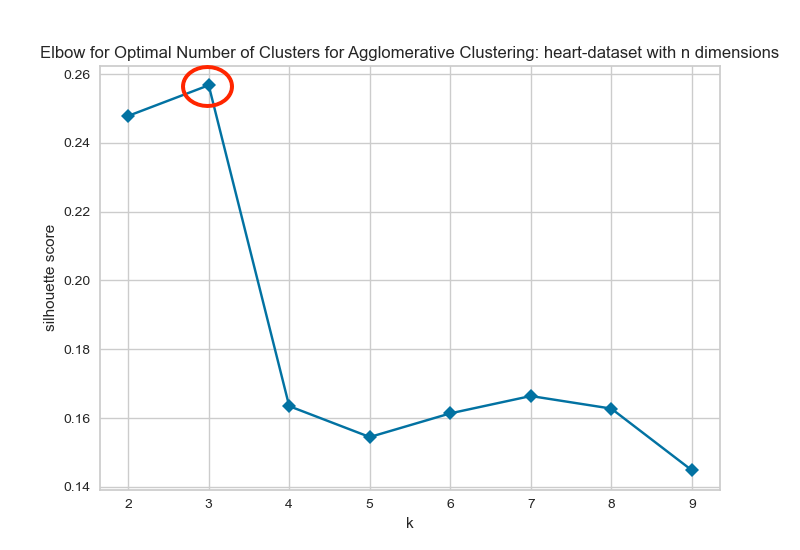
\includegraphics[width=0.75\textwidth]{Method/images/k-values/heart-dataset-n-agglomerative.png}
  \caption{Selecting the $k$ for Agglomerative clustering for Heart dataset (9 dimensions) using the "silhouette method"}
  \label{hyperparameters:agglomerative-heart-dataset-9d}
\end{figure}
\newpage

\subsection{Circle dataset}

\begin{figure}[H]
  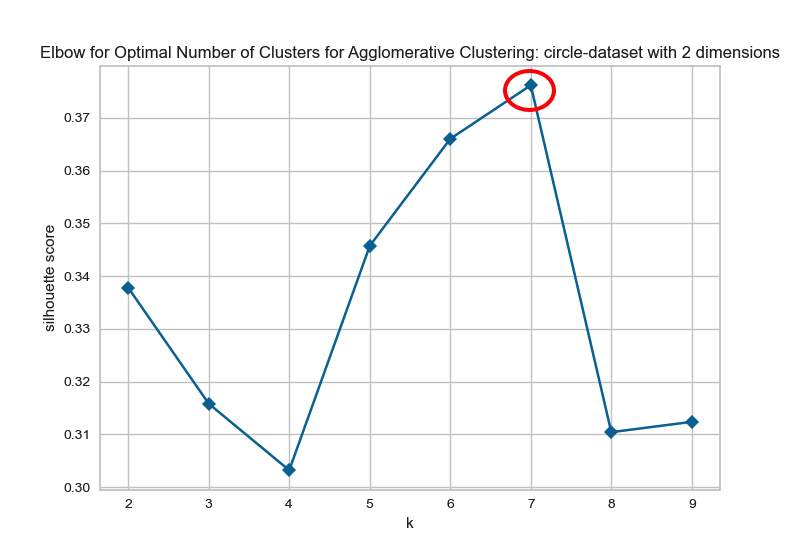
\includegraphics[width=0.75\textwidth]{Method/images/k-values/circle-dataset-2-agglomerative.png}
  \caption{Selecting the $k$ for Agglomerative clustering for circle dataset (2-dimensions) using the "silhouette method"}
  \label{hyperparameters:agglomerative-circle-dataset-2d}
\end{figure}
\begin{figure}[H]
  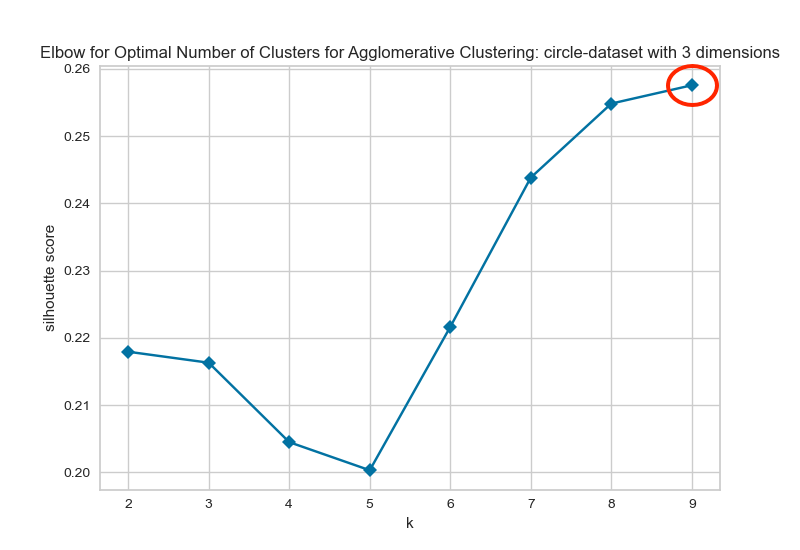
\includegraphics[width=0.75\textwidth]{Method/images/k-values/circle-dataset-3-agglomerative.png}
  \caption{Selecting the $k$ for Agglomerative clustering for circle dataset (3-dimensions) using the "silhouette method"}
  \label{hyperparameters:agglomerative-circle-dataset-3d}
\end{figure}
\newpage

\subsection{Line dataset}
\begin{figure}[H]
  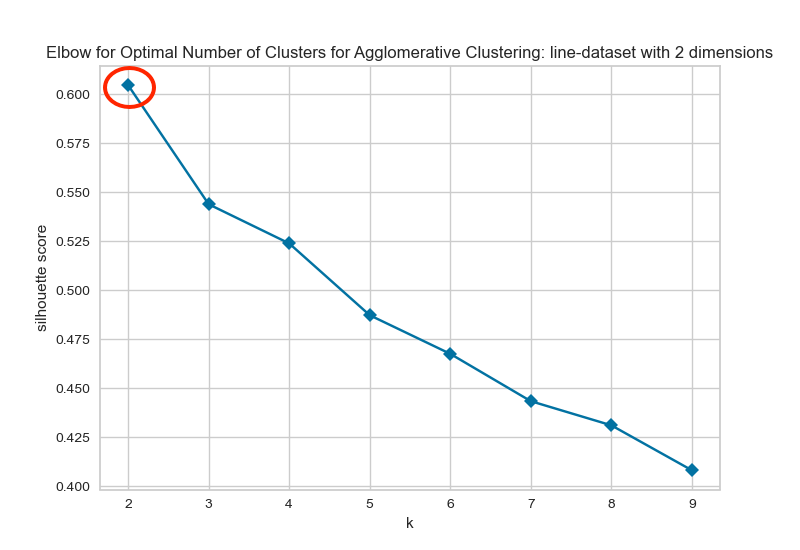
\includegraphics[width=0.8\textwidth]{Method/images/k-values/line-dataset-2-agglomerative.png}
  \caption{Selecting the $k$ for Agglomerative clustering for line dataset (2-dimensions) using the "silhouette method"}
  \label{hyperparameters:agglomerative-line-dataset-2d}
\end{figure}
\begin{figure}[H]
  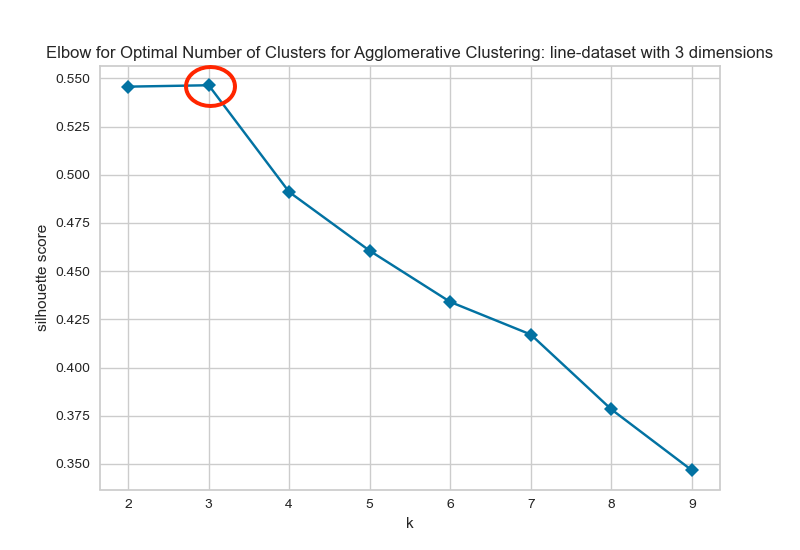
\includegraphics[width=0.75\textwidth]{Method/images/k-values/line-dataset-3-agglomerative.png}
  \caption{Selecting the $k$ for Agglomerative clustering for line dataset (3-dimensions) using the "silhouette method"}
  \label{hyperparameters:agglomerative-line-dataset-3d}
\end{figure}
\newpage
\subsection{Skewed dataset}
\begin{figure}[H]
  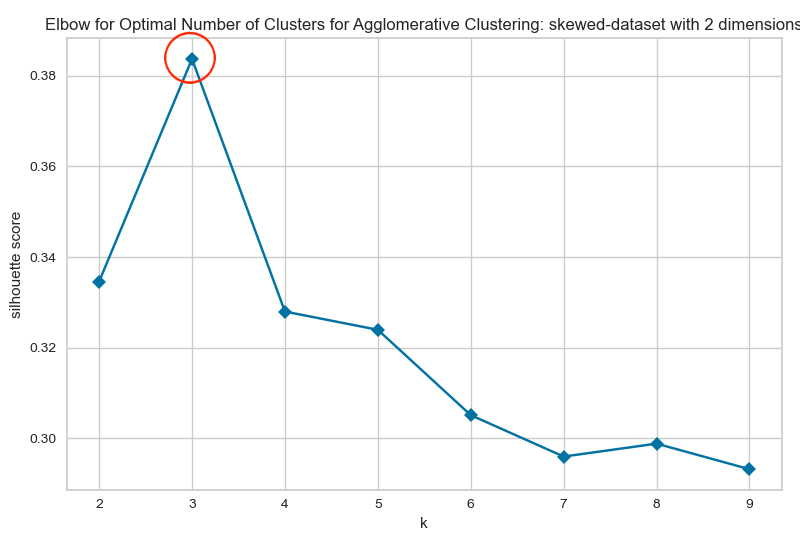
\includegraphics[width=0.75\textwidth]{Method/images/k-values/skewed-dataset-2-agglomerative.png}
  \caption{Selecting the $k$ for Agglomerative clustering for skewed dataset (2-dimensions) using the "silhouette method"}
  \label{hyperparameters:agglomerative-skewed-dataset-2d}
\end{figure}
\begin{figure}[H]
  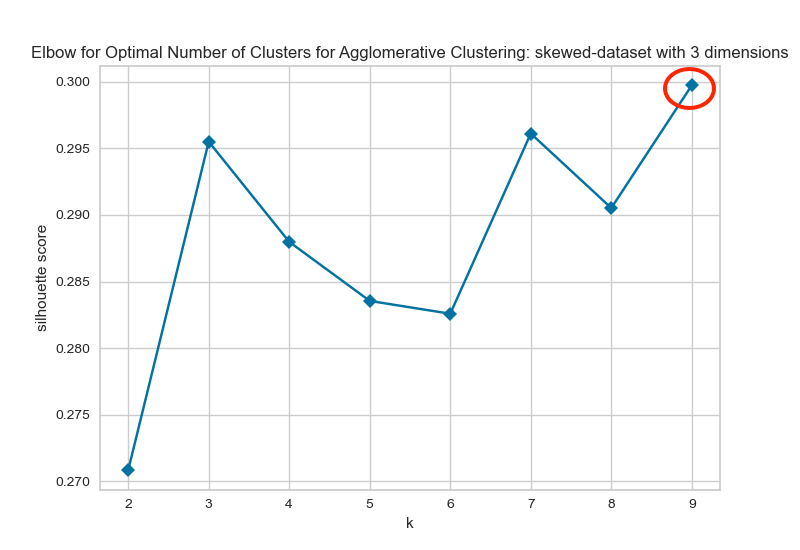
\includegraphics[width=0.75\textwidth]{Method/images/k-values/skewed-dataset-3-agglomerative.png}
  \caption{Selecting the $k$ for Agglomerative clustering for skewed dataset (3-dimensions) using the "silhouette method"}
  \label{hyperparameters:agglomerative-skewed-dataset-3d}
\end{figure}
%  \input{Appendices/appendix-b}
%  \input{Appendices/appendix-c}


\end{document}
